\documentclass[a4paper,12pt]{article}
\usepackage[utf8]{inputenc}
\usepackage[spanish]{babel}
\usepackage{graphicx}
\usepackage{hyperref}
\usepackage{geometry}
\usepackage{longtable}
\usepackage{amsmath}
\usepackage{listings}
\usepackage{xcolor}
\usepackage{fancyhdr}
\usepackage{titlesec}
\usepackage{array}

% Configuración de márgenes
\geometry{top=2.5cm, bottom=2.5cm, left=2.5cm, right=2.5cm}

% Configuración de encabezado y pie de página
\pagestyle{fancy}
\fancyhead{}
\fancyfoot{}
\fancyhead[L]{Sistema de Generación Automática de Exámenes}
\fancyfoot[C]{\thepage}

% Configuración de títulos

\titleformat{\section}{\large\bfseries}{\thesection}{1em}{}
\titleformat{\subsection}{\normalsize\bfseries}{\thesubsection}{1em}{}
\titleformat{\subsubsection}{\normalsize\itshape}{\thesubsubsection}{1em}{}

% Configuración de código fuente
\lstset{
  basicstyle=\ttfamily\footnotesize,
  breaklines=true,
  commentstyle=\color{gray},
  keywordstyle=\color{blue},
  stringstyle=\color{red},
  numbers=left,
  numberstyle=\tiny\color{gray}
}

\begin{document}

\begin{titlepage}
    \centering
    \vspace{1in}
    {\Huge \bfseries Sistema de Generación Automática de Exámenes \par}
    \vspace{1.5in}
    \centering
    \vspace{1in}
    {\Huge \bfseries Autores \par}
    {\Large John García Muñoz - Grupo: 311 CI :03012369124  \par}
    {\Large Victor Hugo Pacheco Fonseca - Grupo: 311 CI :03021580729 \par}
    {\Large Jose Agustín del Toro González - Grupo: 312 CI :01062069124 \par}
    \vfill
    {\Large \today \par}
\end{titlepage}

\tableofcontents
\newpage





\section{Diccionario de datos.}
A continuación mostraremos las principales tablas de la base de datos.

\subsection{User}

\begin{longtable}{| p{3cm} | p{3cm}|p{10cm}|}
	\hline
	\textbf{Campo} & \textbf{Tipo} & \textbf{Descripción} \\
	\hline
	\endfirsthead
	\hline
	\textbf{Campo} & \textbf{Tipo} & \textbf{Descripción} \\
	\hline
	\endhead
	\hline
	\endfoot
	\hline
	\endlastfoot
	
	id & AutoField & Identificador único del usuario \\
	\hline
	password & CharField & Contraseña cifrada del usuario \\
	\hline
	last\_login & DateField & Fecha ultimo inicio de sesión \\
	\hline
	is\_superuser & BoolField & Campo para saber es superusuario \\
	\hline
	email & EmailField & Correo electrónico del usuario \\
	\hline
	first\_name & CharField & Nombre del usuario \\
	\hline
	last\_name & CharField & Primer apellido del usuario \\
	\hline
	last\_name2 & CharField & Segundo Apellido del usuario \\
	\hline
	is\_staff & BoolField &  Acceso al sitio de administración.\\
	\hline
	is\_active & BoolField & Determina si un usuario puede iniciar sesión.\\
	
	\hline
\end{longtable}


\subsection{Teacher}
\begin{longtable}{| p{3cm} | p{3cm}|p{10cm}|}
	\hline
	\textbf{Campo} & \textbf{Tipo} & \textbf{Descripción} \\
	\hline
	\endfirsthead
	\hline
	\textbf{Campo} & \textbf{Tipo} & \textbf{Descripción} \\
	\hline
	\endhead
	\hline
	\endfoot
	\hline
	\endlastfoot
	
	user\_id & ForeingKey & LLave foránea a usuario \\
	\hline
	speciality & CharField & Especialidad del profesor \\
	
\hline
\end{longtable}

\subsection{Student}
\begin{longtable}{| p{3cm} | p{3cm}|p{10cm}|}
	\hline
	\textbf{Campo} & \textbf{Tipo} & \textbf{Descripción} \\
	\hline
	\endfirsthead
	\hline
	\textbf{Campo} & \textbf{Tipo} & \textbf{Descripción} \\
	\hline
	\endhead
	\hline
	\endfoot
	\hline
	\endlastfoot
	
	user\_id & ForeingKey & LLave foránea a usuario \\
	\hline
	age & PosIntegerField & Edad del estudiante \\
	\hline
	course\_id & ForeingKEy & LLave foranea a curso \\
	\hline
	
	\hline
\end{longtable}

\subsection{Course}
\begin{longtable}{| p{3cm} | p{3cm}|p{10cm}|}
	\hline
	\textbf{Campo} & \textbf{Tipo} & \textbf{Descripción} \\
	\hline
	\endfirsthead
	\hline
	\textbf{Campo} & \textbf{Tipo} & \textbf{Descripción} \\
	\hline
	\endhead
	\hline
	\endfoot
	\hline
	\endlastfoot
	
	id & AutoField & Identificador del curso \\
	\hline
	name & CharField & Nombre del curso \\
	\hline
	stard\_date & DateField & Fecha de inicio\\
	\hline
	end\_date & DateField & Fecha de fin\\
	
	\hline
\end{longtable}
\newpage
\subsection{Subject}
\begin{longtable}{| p{3cm} | p{3cm}|p{10cm}|}
	\hline
	\textbf{Campo} & \textbf{Tipo} & \textbf{Descripción} \\
	\hline
	\endfirsthead
	\hline
	\textbf{Campo} & \textbf{Tipo} & \textbf{Descripción} \\
	\hline
	\endhead
	\hline
	\endfoot
	\hline
	\endlastfoot
	
	id & AutoField & Identificador de la asignatura \\
	\hline
	name & CharField & Nombre de la asignatura\\
	\hline
	studyprogram & TextField & Programa de estudio\\
	\hline
	head\_of\_subject\_id & ForeingKey & Identificador del profesor jefe\\
	\hline
	course\_id & ForeingKey & Identificador del curso a la que pertenece\\
	
	\hline
\end{longtable}
 Además se ha creado la tabla \textbf{Subject\_Teacher} , que controla la relacion de ManyToMany entre los modelos subject y teacher.


\subsection{Topic}
\begin{longtable}{| p{3cm} | p{3cm}|p{10cm}|}
	\hline
	\textbf{Campo} & \textbf{Tipo} & \textbf{Descripción} \\
	\hline
	\endfirsthead
	\hline
	\textbf{Campo} & \textbf{Tipo} & \textbf{Descripción} \\
	\hline
	\endhead
	\hline
	\endfoot
	\hline
	\endlastfoot
	
	id & AutoField & Identificador del tema \\
	\hline
	name & CharField & Nombre del tema\\
	\hline
	subject\_id & ForeingKey & Identificador de la asignatura a la que pertenece\\
	
	\hline
\end{longtable}


\subsection{Question}
\begin{longtable}{| p{3cm} | p{3cm}|p{10cm}|}
	\hline
	\textbf{Campo} & \textbf{Tipo} & \textbf{Descripción} \\
	\hline
	\endfirsthead
	\hline
	\textbf{Campo} & \textbf{Tipo} & \textbf{Descripción} \\
	\hline
	\endhead
	\hline
	\endfoot
	\hline
	\endlastfoot
	
	id & AutoField & Identificador de la pregunta \\
	\hline
	content & TextField & Contenido de la pregunta \\
	\hline
	type & CharField & Tipo de pregunta\\
	\hline
	difficulty & CharField & Dificultad de la pregunta\\
	\hline
	date & DateField & Fecha de creación\\
	\hline
	topic\_id & ForeingKey & Identificador del tema al que pertenece\\
	\hline
	teacher\_id & ForeingKey & Identificador del creador de la pregunta\\
	
	\hline
\end{longtable}


\subsection{Exam}
\begin{longtable}{| p{3cm} | p{3cm}|p{10cm}|}
	\hline
	\textbf{Campo} & \textbf{Tipo} & \textbf{Descripción} \\
	\hline
	\endfirsthead
	\hline
	\textbf{Campo} & \textbf{Tipo} & \textbf{Descripción} \\
	\hline
	\endhead
	\hline
	\endfoot
	\hline
	\endlastfoot
	
	id & AutoField & Identificador del exámen \\
	\hline
	type & CharField & Tipo de exámen\\
	\hline
	date & DateField & Fecha de creación\\
	\hline
	subject\_id & ForeingKey & Identificador de la asignatura a la  que pertenece\\
	\hline
	teacher\_id & ForeingKey & Identificador del creador del exámen\\
	\hline
	validteacher\_id & ForeingKey & Identificador del profesor que valida el exámen\\
	\hline
	validation\_date & DateField & Fecha de validación\\
	\hline
	state & CharField & Estado en que se encuentra el exámen \\
	\hline
	
\end{longtable}

 Además se ha creado la tabla \textbf{Exam\_Question} , que controla la relacion de ManyToMany entre los modelos exam y question.
\newpage
\subsection{Observation}
\begin{longtable}{| p{3cm} | p{3cm}|p{10cm}|}
	\hline
	\textbf{Campo} & \textbf{Tipo} & \textbf{Descripción} \\
	\hline
	\endfirsthead
	\hline
	\textbf{Campo} & \textbf{Tipo} & \textbf{Descripción} \\
	\hline
	\endhead
	\hline
	\endfoot
	\hline
	\endlastfoot
	
	id & AutoField & Identificador \\
	\hline
	date & DateField & Fecha de creación \\
	\hline
	exam\_id & ForeingKey & Identificador del exámen\\
	\hline
	ckecked & BoolField & Verificación de revisión\\

	\hline
\end{longtable}



\subsection{AssignedExam}
\begin{longtable}{| p{3cm} | p{3cm}|p{10cm}|}
	\hline
	\textbf{Campo} & \textbf{Tipo} & \textbf{Descripción} \\
	\hline
	\endfirsthead
	\hline
	\textbf{Campo} & \textbf{Tipo} & \textbf{Descripción} \\
	\hline
	\endhead
	\hline
	\endfoot
	\hline
	\endlastfoot
	
	id & AutoField & Identificador  \\
	\hline
	type & CharField & Tipo de exámen  \\
	\hline
	exam\_id & ForeingKey & Identificador del exámen. \\
	\hline
	date & DateField & Fecha de asignación\\
	
	\hline
\end{longtable}

\subsection{ExamDone}
\begin{longtable}{| p{3cm} | p{3cm}|p{10cm}|}
	\hline
	\textbf{Campo} & \textbf{Tipo} & \textbf{Descripción} \\
	\hline
	\endfirsthead
	\hline
	\textbf{Campo} & \textbf{Tipo} & \textbf{Descripción} \\
	\hline
	\endhead
	\hline
	\endfoot
	\hline
	\endlastfoot
	
	id & AutoField & Identificador del exámen hecho \\
	\hline
	date & DateField & Fecha del exámen hecho \\
	\hline
	student\_id & ForeingKey & Identificador del estudiante\\
	\hline
	exam\_id & ForeingKey & Identificador del exámen\\
	\hline
\end{longtable}


\subsection{ExamQuestionResponse}
\begin{longtable}{| p{3cm} | p{3cm}|p{10cm}|}
	\hline
	\textbf{Campo} & \textbf{Tipo} & \textbf{Descripción} \\
	\hline
	\endfirsthead
	\hline
	\textbf{Campo} & \textbf{Tipo} & \textbf{Descripción} \\
	\hline
	\endhead
	\hline
	\endfoot
	\hline
	\endlastfoot
	
	id & AutoField & Identificador de la respuesta de la pregunta  \\
	\hline
	question\_id & ForeingKey & Identificador del la pregunta\\
	\hline
	exam\_done\_id & ForeingKey & Identificador del exámen hecho \\
	\hline
	response & TextField & Respuesta de la pregunta  \\
	\hline
	note & IntegerField & Nota de la respuesta \\
	
	\hline
\end{longtable}


\subsection{ExamGrade}
\begin{longtable}{| p{3cm} | p{3cm}|p{10cm}|}
	\hline
	\textbf{Campo} & \textbf{Tipo} & \textbf{Descripción} \\
	\hline
	\endfirsthead
	\hline
	\textbf{Campo} & \textbf{Tipo} & \textbf{Descripción} \\
	\hline
	\endhead
	\hline
	\endfoot
	\hline
	\endlastfoot
	
	id & AutoField & Identificador  \\
	\hline
	date & DateField & Fecha de la calificación\\
	\hline
	exam\_done\_id & ForeingKey & Identificador del exámen hecho \\
	\hline
	teacher\_id & ForeingKey & Identificador del profesor que revisó \\
	\hline
	finalnote & IntegerField & Nota final del exámen \\
	
	\hline
\end{longtable}

\subsection{ReevaluatedExam}
\begin{longtable}{| p{3cm} | p{3cm}|p{10cm}|}
	\hline
	\textbf{Campo} & \textbf{Tipo} & \textbf{Descripción} \\
	\hline
	\endfirsthead
	\hline
	\textbf{Campo} & \textbf{Tipo} & \textbf{Descripción} \\
	\hline
	\endhead
	\hline
	\endfoot
	\hline
	\endlastfoot
	
	id & AutoField & Identificador de la recalificación  \\
	\hline
	exam\_grade\_id & ForeingKey & Identificador del exámen calificado \\
	\hline
	teacher\_id & ForeingKey & Identificador del profesor que revisó \\
	\hline
	note & IntegerField & Nota de la recalificación\\
	
	\hline
\end{longtable}



\section{Esquema con el diseño de la aplicación}
La aplicación sigue un flujo cliente-servidor, donde el frontend (React) y el backend (Django Rest
Framework) se comunican a través de solicitudes HTTP.
\newline

\subsection{Backend}

\textbf{Componentes principales}
\begin{itemize}
	
	\item \textbf{Modelos}:Definidos en models.py, representan las estructuras de datos y tablas en la base de datos.
	\item \textbf{Serializadores}:Definidos en serializers.py, transforman instancias de modelos en formatos como JSON, y viceversa.
	\item \textbf{Vistas(Views)}: Definidas en views.py, manejan las solicitudes HTTP y devuelven respuestas adecuadas.
		\item \textbf{URLs}:Configuradas en urls.py, mapean las rutas a las vistas correspondientes.
	\item \textbf{Informes y Estadísticas}: Ofrece informes sobre la utilización de preguntas, el desempeño de los estudiantes y la distribución de preguntas por tema y dificultad, lo que facilita la toma de decisiones informadas.
\end{itemize}




\section{Diagrama de Clases}
\subsection{Usuario}
\begin{itemize}
    \item Puede ser un profesor o estudiante.
    \item Relacionado con Curso (Muchos a uno para los estudiantes).
	\item Crea Preguntas y Exámenes (para los profesores).
	\item Realiza Intentos de Exámen (para los estudiantes).
	\item Realiza Calificaciones (para los profesores).
\end{itemize}

\subsection{Curso}
\begin{itemize}
	\item Relación Uno a Muchos con Usuario (estudiantes).
	\item Contiene varias Asignaturas.
\end{itemize}

\subsection{Asigantura}
\begin{itemize}
	\item Pertenece a un Curso.
	\item Contiene varios Temas y Exámenes.
\end{itemize}

\subsection{Tema}
\begin{itemize}
	\item Pertenece a una Asignatura.
	\item Contiene varias Preguntas.
\end{itemize}

\subsection{Exámen}
\begin{itemize}
	\item Pertenece a una Asignatura.
	\item Contiene varias Preguntas. Relación Muchos a Muchos
	\item Es creada y validada por un Profesor.
	\item Contiene Observaciones.
\end{itemize}

\subsection{Observación}
\begin{itemize}
	\item Asociado a una Exámen. Relación Muchos a Uno.
\end{itemize}

\subsection{Asignación de  Exámen}
\begin{itemize}
	\item Asociado a una Exámen. 
\end{itemize}

\subsection{ExamDone}
\begin{itemize}
	\item Es realizado por un estudiante.
	\item Está asociado a un Exámen.
	\item Es creada y validada por un Profesor.
	\item Asociado a una Calificación.
\end{itemize}

\subsection{ExamQuestionResponse}
\begin{itemize}
	\item Asociado a un exámen hecho.
	\item Asociado a una pregunta.
\end{itemize}

\subsection{ExamGrade(Calificación)}
\begin{itemize}
	\item Está asociada a un ExamDone. Relación Uno a Uno
	\item Es realizada por un Profesor.
	\item Asociado a una Recalificación.
\end{itemize}

\subsection{ReevaluatedExam(Recalificación)}
\begin{itemize}
	\item Está asociada a una calificación(ExamGrade). Relación Uno a Uno
	\item Es realizada por un Profesor.
\end{itemize}

\section{Esquema de las clases definidas}
 En la siguiente figura se muestra un esquema de las clases definidas.

\begin{figure}[h]  % El entorno figure facilita la colocación y manejo de las imágenes
	\centering     % Centra la imagen
	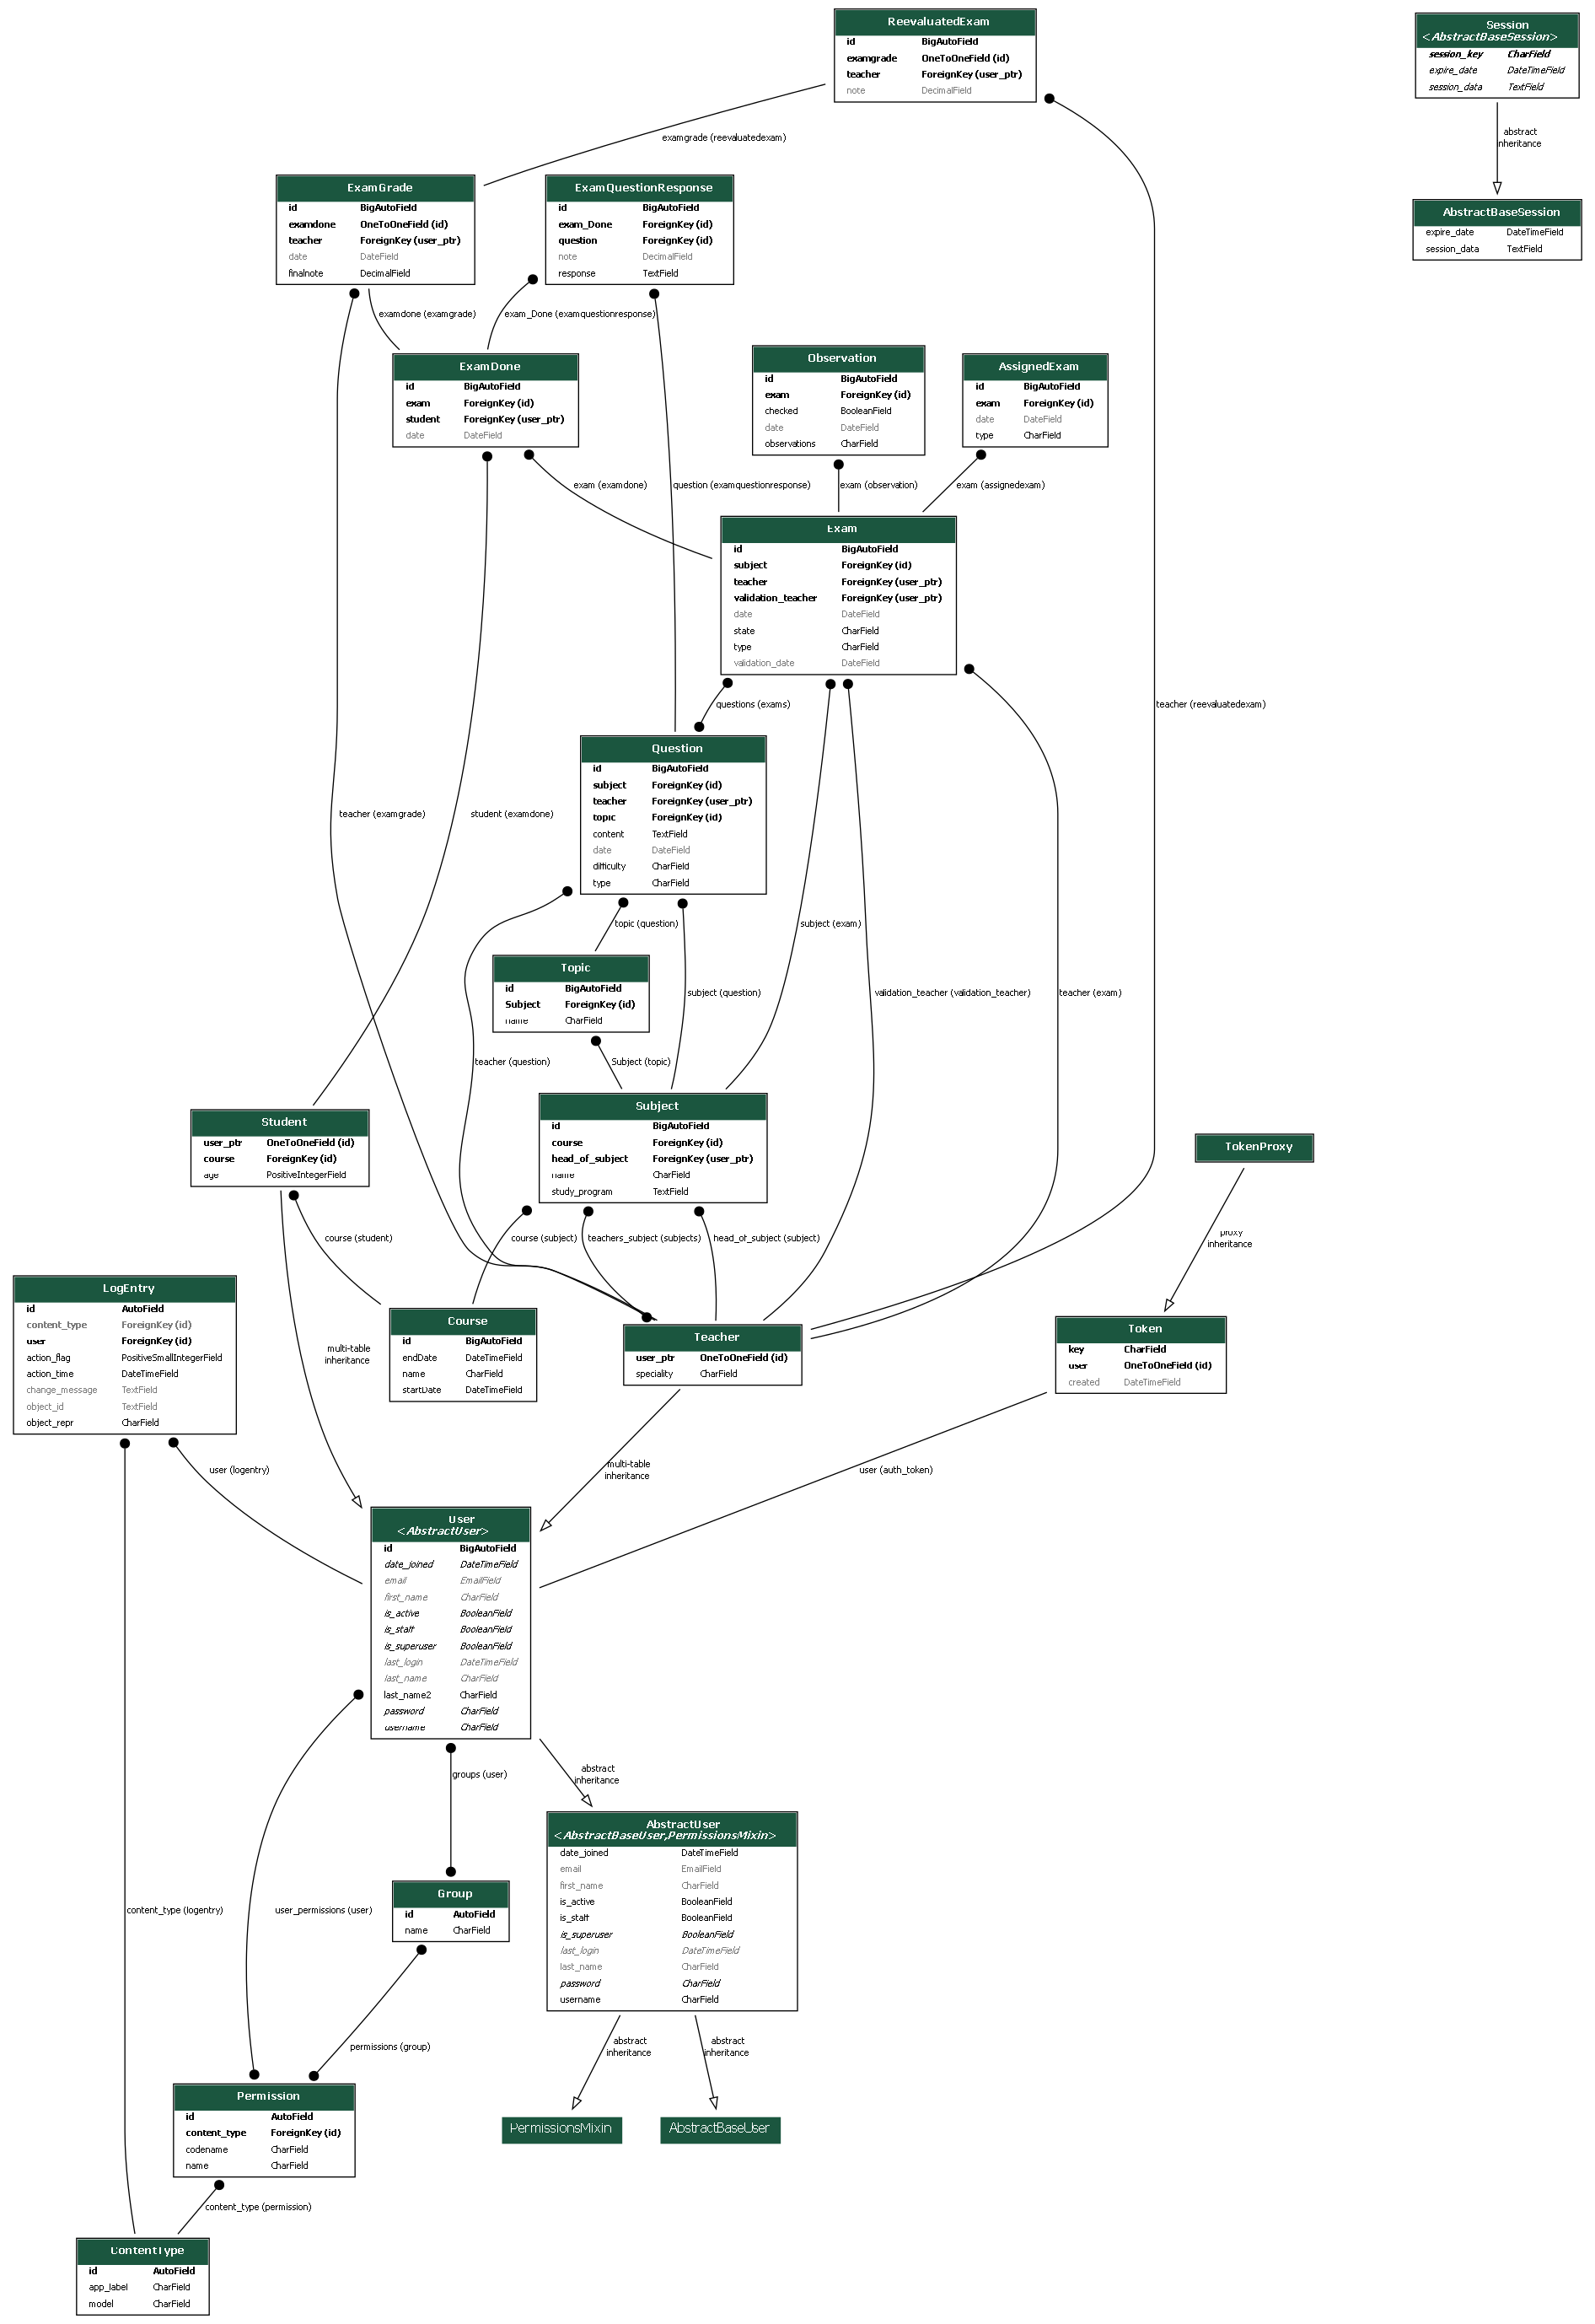
\includegraphics[width=0.5\textwidth]{my_project_visualized.png}
	\caption{Esquema de las clases definidas.}
	\label{fig:mi_imagen}
\end{figure}


\section{Solución Propuesta}
Se utilizó una Arquitectura compuesta por:

\begin{itemize}
	\item Capa de Presentación (Frontend): Construida con React, proporciona una interfaz de usuario interactiva y dinámica para la interacción con el sistema.
	\item Capa de Lógica de Negocio (Backend): Implementada con Django REST Framework, maneja la lógica de aplicación, controla el flujo de datos entre el frontend y la base de datos, y aplica las reglas de negocio.
	\item Capa de Datos (Base de Datos): SQLite como base de datos, ya que es ligera y suficiente para un
	entorno de desarrollo no destinado a producción.
\end{itemize}

\subsection{Descripción de los Módulos}
\subsection{Módulo de Autenticación}
\begin{itemize}
	\item Maneja el registro, inicio de sesión y control de acceso de los usuarios.
	\item Implementa JWT (JSON Web Tokens) para la autenticación segura de usuarios.
	
\end{itemize}
\subsection{Módulo de Gestión de Preguntas}
\begin{itemize}
	\item Permite a los profesores crear, actualizar y eliminar preguntas .
	\item Permite al administrador crear, actualizar y eliminar asignaturas y temas .
	\item Proporciona endpoints para listar y obtener detalles de las asignaturas ,temas, y preguntas.
	
	
\end{itemize}

\subsection{Módulo de Gestión de Exámenes}
\begin{itemize}
	\item Permite la creación y validación de exámenes, seleccionando preguntas existentes.
	\item  Permite que los estudiantes pueden realizar exámenes asignados y enviar sus respuestas.
	\item Los profesores pueden calificar y recalificar exámenes, proporcionando feedback a los estudiantes.
	\item Proporciona endpoints para listar y obtener detalles de exámenes ,calificación y recalificación .
\end{itemize}

\subsection{Módulo de Reportes y Exportación de Datos}
\begin{itemize}
	\item Permite la generación de informes detallados sobre el desempeño de estudiantes, exámenes realizados, etc.
	\item  Implementa funcionalidades para exportar datos en formatos como CSV y PDF.

\end{itemize}


\section{Información Adicional para el Mantenimiento del Sistema}
Para preguntas adicionales o soporte, contactar con el equipo de desarrollo a través de pachecovictorh003@gmail.com.

\end{document}


